\documentclass{article}
\usepackage[left=2cm,right=2cm,top=2cm,bottom=2cm]{geometry}
\usepackage[utf8]{inputenc}
\usepackage[german]{babel}
\usepackage{amsmath}
\usepackage{dsfont}
\usepackage[export]{adjustbox}
\usepackage{amsthm}
\usepackage{color}
\usepackage{amsfonts}
\usepackage{amssymb}
\usepackage{wasysym}
\usepackage{makeidx}
\usepackage{graphicx}
\usepackage[colorlinks=true,urlcolor=blue,linkcolor=blue]{hyperref}
\usepackage{ziffer}
\usepackage{minted}
\usepackage{xcolor}
\usepackage{framed}
\usepackage{mdframed}
\usepackage{subfiles}
\usemintedstyle{emacs}

\definecolor{purp}{HTML}{9A72AC}
\definecolor{re}{HTML}{FC6255}
\definecolor{gre}{HTML}{83C167}
\definecolor{blu}{HTML}{58C4DD}
\definecolor{shadecolor}{rgb}{0.85,0.85,0.85}
\definecolor{bg}{rgb}{0.95,0.95,0.95}
\setlength{\parindent}{0em} 

\BeforeBeginEnvironment{minted}{\begin{mdframed}[linewidth =2 ,backgroundcolor=bg , linecolor=black, linewidth=0.5]}
\AfterEndEnvironment{minted}{\end{mdframed}}

\newtheorem{defi}{Definition}
\BeforeBeginEnvironment{defi}{\begin{mdframed}[linewidth =2 ,backgroundcolor=bg , linecolor=black, linewidth=0.5]}
\AfterEndEnvironment{defi}{\end{mdframed}}

\newcommand{\bsp}{\textbf{Beispiel}:}
%\newcommand{\task}{\textbf{Aufgabe}:}

\newcommand{\bol}[1]{\textbf{#1}}
\newcommand{\q}[1]{\glqq #1\grqq}
\newcommand{\DODO}[1]{\textbf{\textcolor{red}{DODO:}} #1 \\ \begin{center}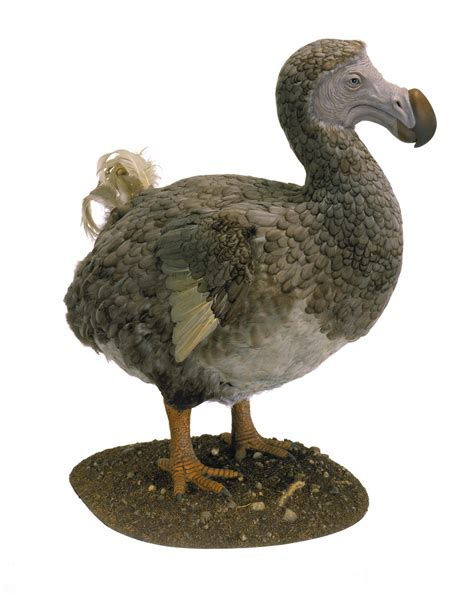
\includegraphics[scale=0.2]{../../media/dodo.jpg} \end{center}}

\newenvironment{task}[1]{
    \begin{shaded*}
    \textbf{Aufgabe #1}:
}{
    \end{shaded*}
}

\begin{document}
Eine zweite - wenn auch nicht so häufig verwendete - Möglichkeit der Implementierung ist die Verwendung von \textbf{Adjazenzlisten}. Die grundlegende Idee besteht dabei darin, für jeden Knoten eine Liste der anderen Knoten zu speichern. Da bei uns auch Kantengewichte repräsentiert werden sollen, können nicht einfach die Knoten, die von einem Knoten aus erreicht werden können in einem Array gespeichert werden. Ein Array wäre ohnehin für unseren Verwendungszweck ungeeignet, da wir Kanten hinzufügen und gegebenenfalls auch löschen wollen. \\
Jeder Eintrag der Liste repräsentiert also eine Kante und speichert das Gewicht und den Knoten zu dem diese Kante zeigt als Referenz in einem Attribut. Der Startknoten muss nicht gespeichert werden, wenn wir die Adjazenlisten in den einzelnen Knoten verwalten. Soll nur die Graph-Klasse alle Adjazenzlisten kennen, so könnte der Einfachheit halber der Startknoten zusätzlich gespeichert werden. Wie immer ein Klassendiagramm - diesmal auch mit den entsprechenden grundlegenden Methoden: 
\begin{center}
    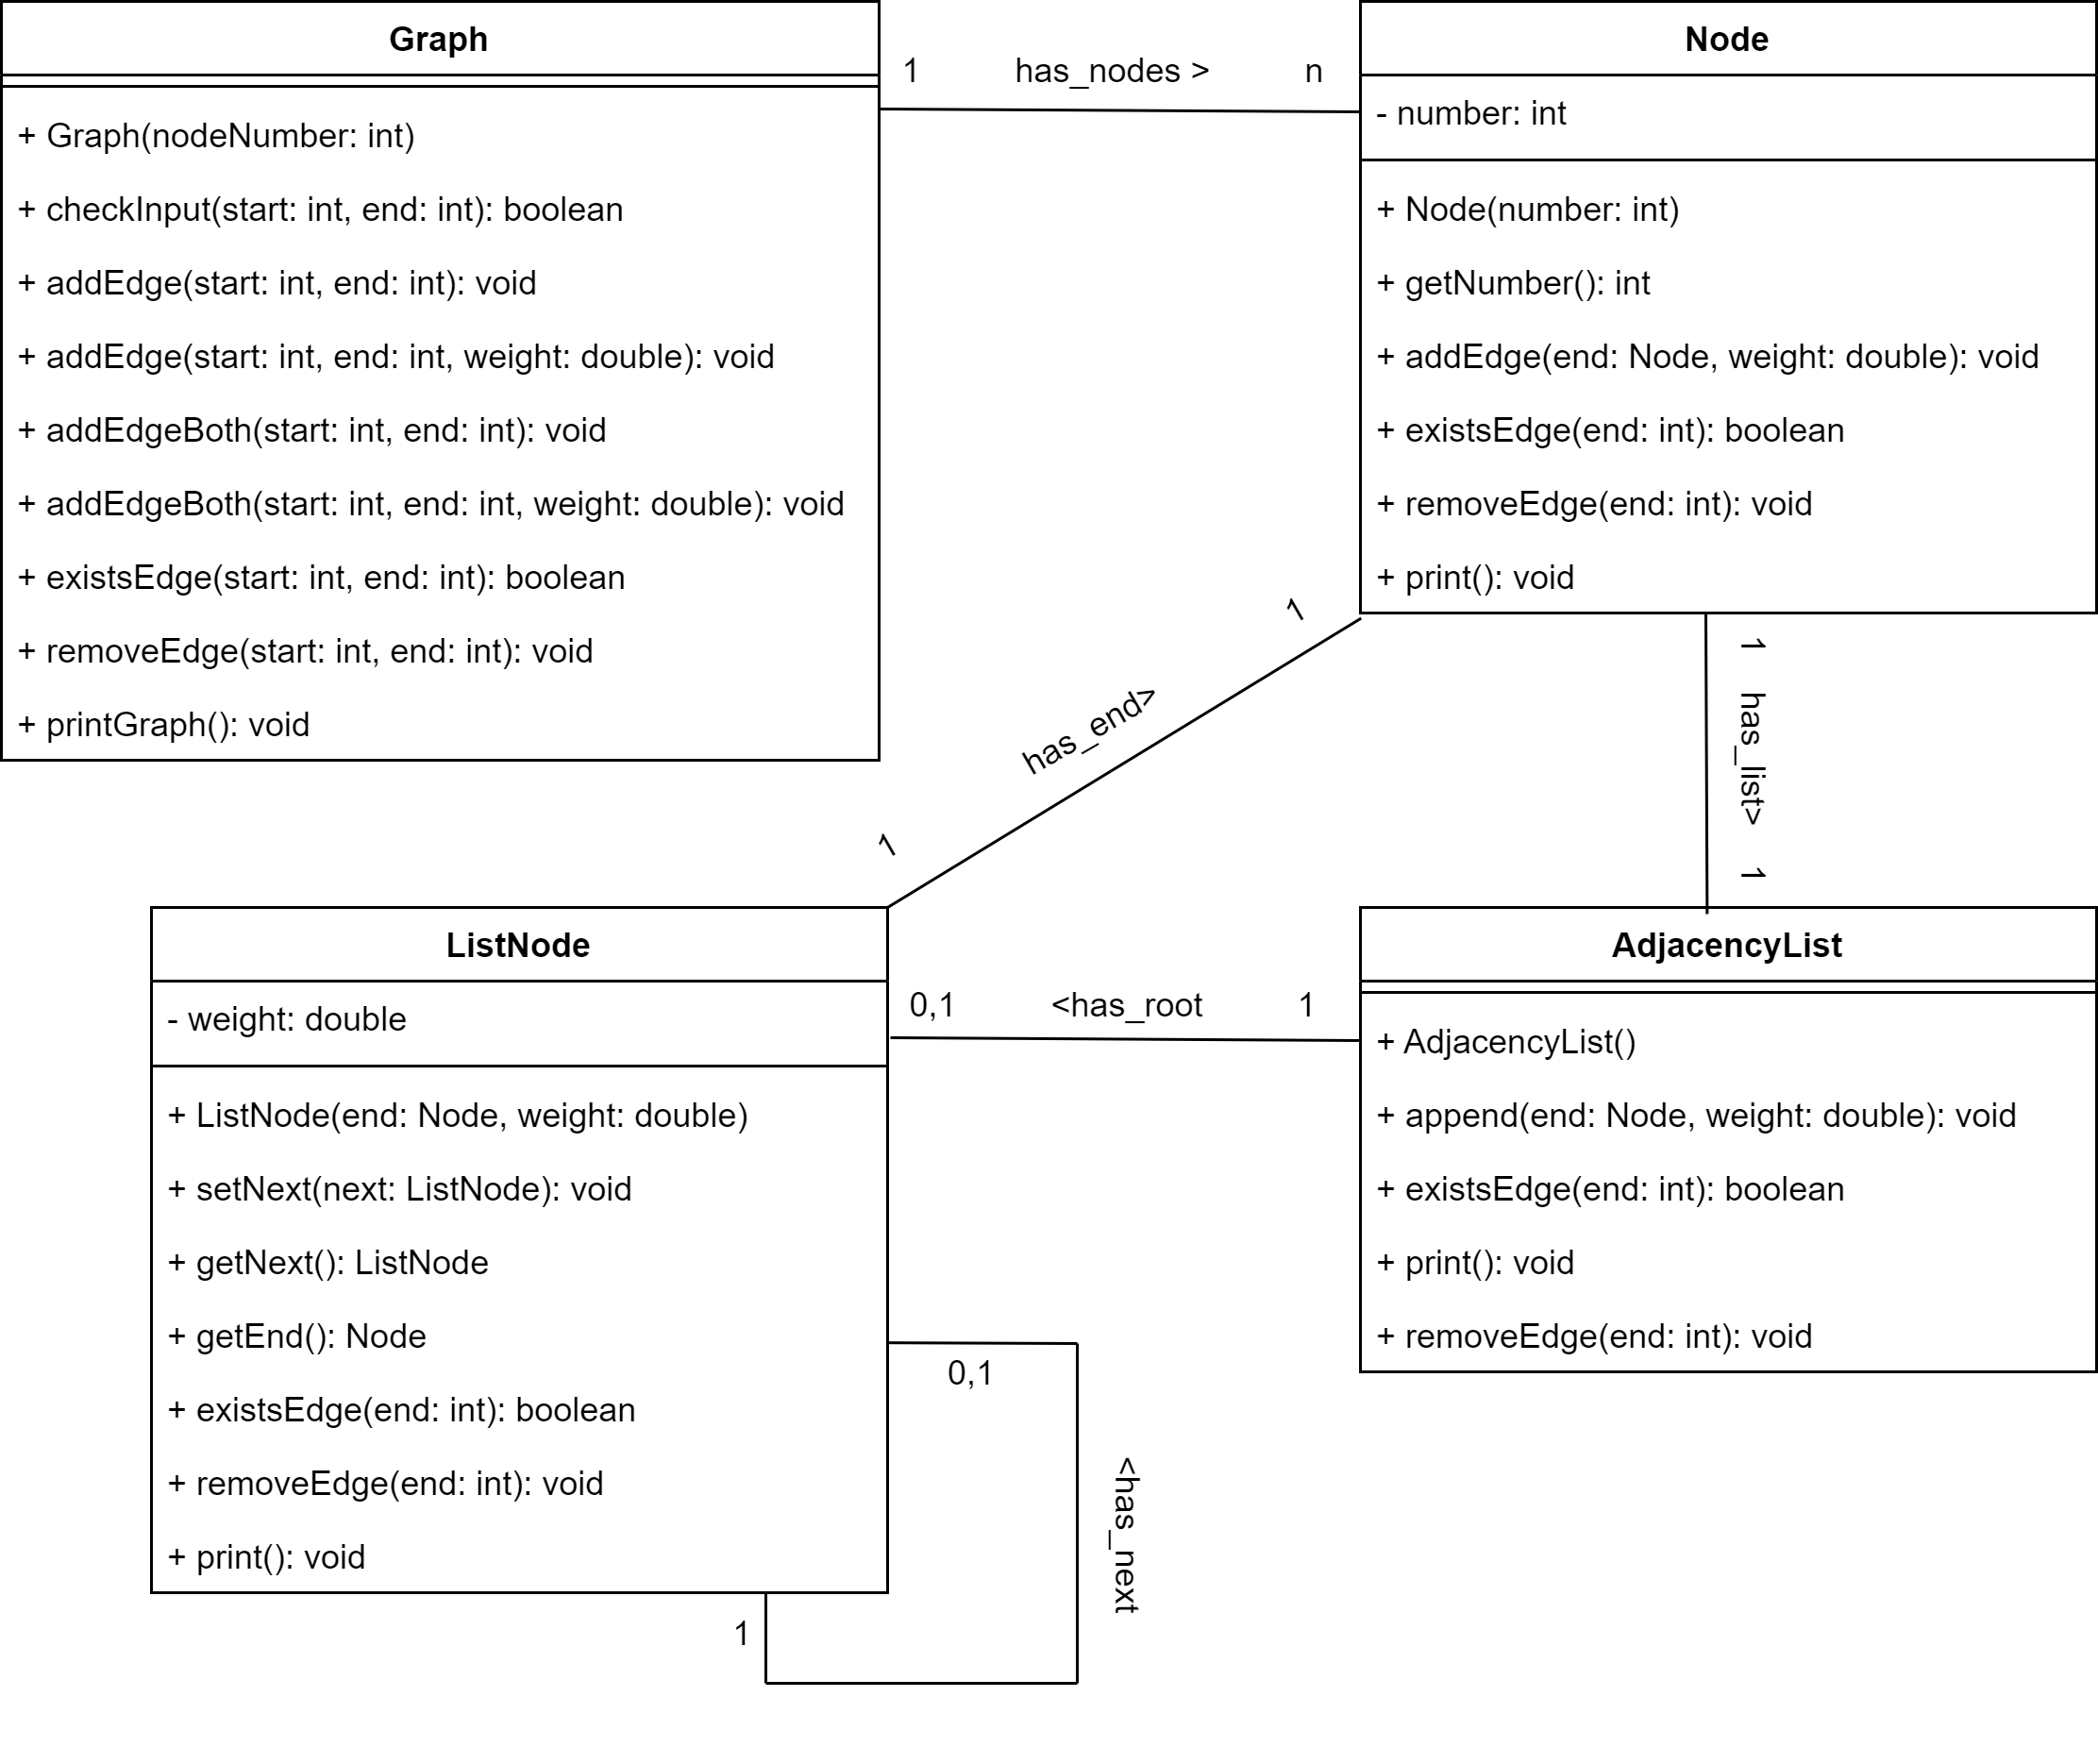
\includegraphics[scale=0.2]{../media/graphs_lists.png}
\end{center}
\textbf{Hinweis:} Die Adjazenzliste ist in dieser Implementierung nicht mit einem Kompositum versehen, da diese nicht viel \q{können} muss. Das Einfügen der zusätzlichen Klassen rechtfertigt weder den Schreibaufwand, noch verbessert es die Performance. Auch der Überblick ist mit den wenigen Methoden nicht gefährdet. 
\begin{task}{- Die Einzige hier}
    Implementieren Sie das oben stehende Klassendiagramm.
\end{task}

\newpage

Nachfolgend die Lösung, jeweils geordnet nach Klassen mit Kommentaren:

\begin{minted}{java}
public class Graph {
    private Node[] nodes;

    //Analog zur anderen Implementierung
    public Graph(int nodeNumber) {
        if(nodeNumber <= 0) {
            nodeNumber = 5;
        }
        nodes = new Node[nodeNumber];
        for(int i = 0; i < nodes.length; i++) {
            nodes[i] = new Node(i);
        }
    }

    public boolean checkInput(int start, int end) {
        if(start < 0 || start >= nodes.length || end < 0 || end >= nodes.length) {
            System.out.println("Hier kann es keine Kante geben!");
            return false;
        }
        return true;
    }

    //Im Gegensatz zu vorher müssen wir bei allen Methoden auf dem Startknoten der
    //Kante eine Methode aufrufen, damit für die Adjazenzliste gegebenenfalls
    //ebenfalls eine passende Methode gestartet wird.
    public void addEdge(int start, int end) {
       if(checkInput(start, end)) nodes[start].addEdge(nodes[end], 0);
    }

    //Hier nur zusätzlich mit Gewicht!
    public void addEdge(int start, int end, double weight) {
        if(checkInput(start, end)) nodes[start].addEdge(nodes[end], weight);
    }

    public void addEdgeBoth(int start, int end) {
        if(checkInput(start, end)) {
            nodes[start].addEdge(nodes[end], 0);
            nodes[end].addEdge(nodes[start], 0);
        }
    }

    public void addEdgeBoth(int start, int end, double weight) {
        if(checkInput(start, end)) {
            nodes[start].addEdge(nodes[end], weight);
            nodes[end].addEdge(nodes[start], weight);
        }
    }

    public boolean existsEdge(int start, int end) {
        if(!checkInput(start, end)) return false;
        if(nodes[start].existsEdge(end)) {
            return true;
        }
        return false;
    }

    public void removeEdge(int start, int end) {
        if(checkInput(start, end)) {
            nodes[start].removeEdge(end);
        } 
    }
    //for(Type t : array) - eine Kurzschreibweise, mit der alle Einträge
    // eines Arrays durchlaufen werden, man könnte es auch "for each element ..." nennen.
    public void printGraph() {
        for(Node node : nodes) {
            node.print();
            System.out.println();
        }
    }
}
\end{minted}
\begin{minted}{java}
public class Node {
    private int number;
    private AdjacencyList adjL;

    //Jeder Knoten kennt seine Nummer und hat eine Adjazenzliste, die am Anfang leer ist.
    public Node(int number) {
        this.number = number;
        adjL = new AdjacencyList();
    }

    //Alle weiteren Methoden "leiten" nur zur Adjazenzliste weiter.
    public void addEdge(Node end, double weight) {
        adjL.append(end, weight);
    }

    public boolean existsEdge(int end) {
        return adjL.existsEdge(end);
    }

    public void removeEdge(int end) {
        adjL.removeEdge(end);
    }

    public int getNumber() {
        return number;
    }

    public void print() {
        System.out.println("This is node number " + number + " and here are my neighbours: ");
        adjL.print();
    }
}
\end{minted}
\begin{minted}{java}
public class AdjacencyList {
    private ListNode root;

    //Wie oben bereits erwähnt ist dies eine Liste mit null-Referenz am Ende!
    public AdjacencyList() {
        root = null;
    }

    //Wir fügen vorne an, da dies laufzeittechnisch besser ist und Reihenfolge
    //für uns keine Rolle spielt!
    public void append(Node end, double weight) {
        if(root != null) {
            ListNode tmp = new ListNode(end, weight);
            tmp.setNext(root);
            root = tmp;
        } else {
            root = new ListNode(end, weight);
        }
        
    }

    //Die folgenden Methoden steuern jeweils wieder eine Rekursion
    public boolean existsEdge(int end) {
        if(root != null) {
            return root.existsEdge(end);
        }
        return false;
    }

    public void removeEdge(int end) {
        if(root != null) {
            if(root.getEnd().getNumber() == end) {
                root = root.getNext();
            } else {
                root.removeEdge(end);
            }
        } else {
            System.out.println("This node has no edges to delete");
        }
    }

    public void print() {
        if(root != null) {
            root.print();
        }
    }
}
\end{minted}
\begin{minted}{java}
public class ListNode {
    private Node end;
    private double weight; 
    private ListNode next;

    //Es würde auch nichts dagegen sprechen verschiedene Gewichte zu speichern, 
    //dann müsste allerdings auch die Interaktion mit der Kante anders modelliert werden.
    public ListNode(Node end, double weight) {
        this.end = end;
        this.weight = weight;
        this.next = null;
    }

    public void setNext(ListNode next) {
        this.next = next;
    }

    public ListNode getNext() {
        return next;
    }

    public Node getEnd() {
        return end;
    }

    //Die folgenden Methoden entsprechen von der Struktur der Rekursion genau unserer 
    //ersten LinkedList
    public boolean existsEdge(int end) {
        if(this.end.getNumber() == end) {
            return true;
        } 
        if(next == null) {
            return false;
        }
        return next.existsEdge(end);
    }

    public void removeEdge(int end) {
        if(next == null) {
            System.out.println("There is no edge to remove here");
        }
        if(next.getEnd().getNumber() == end) {
            next = next.getNext();
        }
    }

    public void print() {
        System.out.println("Neighbour: " + end.getNumber() + " with weight " + weight);
        if(next != null) {
            next.print();
        }
    }
}
\end{minted}
\end{document}